\section{Auswertung}
\label{sec:auswertung}

\subsection{Zählrohr Charakterristik}
\label{sec:characteristik}

\begin{figure}
    \centering
    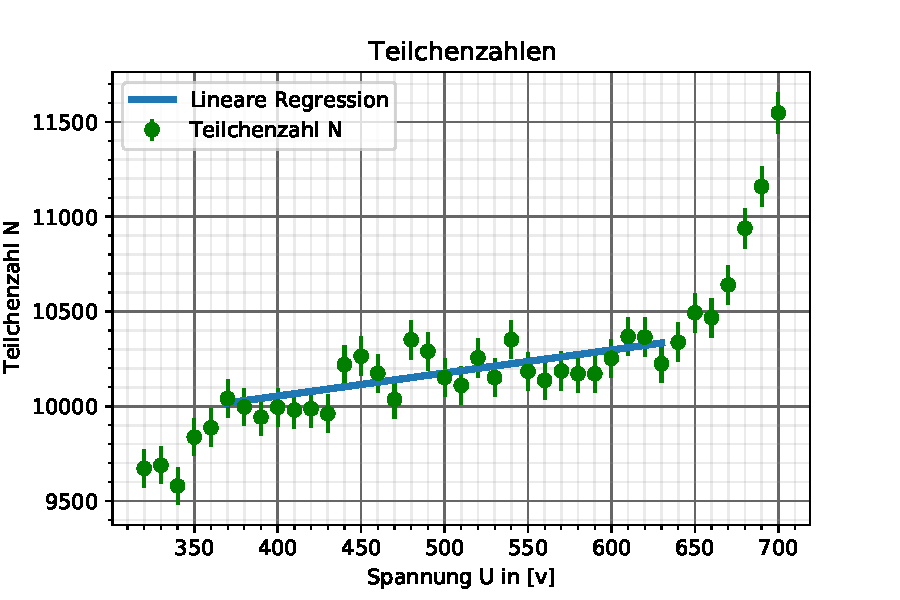
\includegraphics{kennlinie.pdf}
    \caption{Teilchenzahlen im Geiger-Müller-Zählrohr}
    \label{fig:teilchenzahl}
  \end{figure}
Um die Plateau-Steigung zu ermittlen wurde mittels linearer Regression ein polynom ersten Grades der 
Form $f(x)=ax+b$ durch die Messpunkte gelegt:
\begin{center}
    $f(x)=(1.215\pm0.256)x + (9567.924\pm125.414)$ $\rightarrow$ $D_f=\{x\in\mathbb{R} \vert 360\le x\le620\}$    
\end{center}
Das Plateau hat eine Länge von etwa $\SI{260}{V}$ im Bereich von $\SI{360}{V}$ bis $\SI{620}{V}$ und  eine 
Steigung von $\SI{1,215\pm0,256}{\frac{\%}{100}}$.
\subsection{Totzeit des Zählrohres}
\label{sec:totzeit}
\subsubsection{Totzeitbestimmung mit dem Oszilloskop}
\label{sec:totzeitO}
\subsubsection{Totzeitbestimmung mit der Zwei-Quellen-Methode}
\label{sec:totzeitZ}
\subsection{Ladung pro einfallendem Teilchen}
\label{sec:ladung}
